%!TEX root = dippa.tex
%%% This file contains the MicroRNAs section of my master's thesis.
%%% This section covers the biological background of miRNAs.
%%% Author: Viljami Aittomäki

\section{MicroRNAs}\label{micrornas}

MicroRNAs (miRNAs) are a family of endogenous (i.e. coming from within the
cell itself) noncoding small RNA molecules that function as post-transcriptional
regulators of gene expression \citep{Ambros2004}. In their
functional, mature form miRNAs are single stranded and approximately 22
nucleotides long. MicroRNAs are not translated into protein. Instead, they
have an important role in regulation of gene expression in a wide range of
physiological, developmental and pathological processes \citep{Bartel2009}.
MicroRNAs assert their regulatory function by destabilization and degradation
of target messenger RNA (mRNA) molecules and inhibition of mRNA translation
\citep{Fabian2010}.




\subsection{Discovery of microRNAs}

The first known microRNA, lin-4, was discovered in 1993 by two research groups
studying the larval development of the nematode \emph{Caenorhabditis elegans}.
The researchers noted that lin-4 does not encode a protein, but instead
produces a pair of small RNAs, the longer of which was proposed to be a
precursor to the shorter one \citep{Lee1993}. The RNAs encoded by lin-4 were
noted to have conserved antisense complementarity in several sites of an
untranslated region of the lin-14 mRNA, and these sites were found to be
necessary for the normal repression of lin-14 expression by lin-4
\citep{Lee1993,Wightman1993}.
%It
%should be noted, that one of these groups also showed that lin-4 reduces the
%amount of the LIN-14 protein -- the end-product of the lin-14 gene -- without
%significantly affecting the cellular concentration of the lin-14 mRNA
%\citep{??}. %oks tää Wightman1993:ssa?
%We will return to the issue of microRNA action in chapter \ref{microrna-function}.

Let-7, the second microRNA to be discovered, was also first found in \emph{C.
elegans}, however, homologues of let-7 were found in several other species
\citep{Pasquinelli2000}. Soon after, numerous microRNA genes were found across
a variety of species, and a registry was set up to serve as a comprehensive
knowledge base of published microRNAs and as an independent authority on
microRNA nomenclature \citep{GriffithsJones2004}. This registry later became
miRBase, the de facto reference database of known microRNAs, and now provides
sequence data, annotations as well as predicted and validated target genes for
miRNAs \citep{Kozomara2014}.

The number of known small RNAs has since vastly expanded
and microRNAs have been found in more than 200 organisms, including
all studied animals, plants \citep{JonesRhoades2006} and viruses \citep{Grundhoff2011}. 
The number of records in miRBase has risen exponentially
from %218 precursor and
218 mature miRNAs in the first release in 2002 to %28645 precursor and
35828 mature miRNAs in 223 species in the most recent version (v21, released June
2014 \citep{VanPeer2014,MiRBaseWeb}), illustrating the vast amount of novel
microRNA molecules discovered recently, mainly due to increasing efforts in
and availability of sequencing. miRBase lists 2588 known human miRNAs at the
time of writing this thesis. A web service called miRBaseTracker has been
developed by \citet{VanPeer2014} for updating miRNA nomenclature and
annotations across different versions of miRBase to allow correct comparison
of miRNA study results and reannotation of miRNA analysis platforms.




\subsection{MicroRNA genomics}\label{microrna-genomics}

MicroRNAs are highly conserved in evolution \citep{Bartel2004}, for example,
55\% of \emph{C. elegans} miRNAs have homologues in humans
\citep{IbanezVentoso2008}. Interestingly, the
appearance of multi-cellular organisms appears to correlate with the
appearance of the microRNA machinery, and organism complexity and speciation
are correlated with miRNA complexity, suggesting that microRNAs have had a
crucial role in the development of complex organisms \citep{Lee2007}.

MicroRNAs are found in varying genomic contexts. Approximately 50\% of
mammalian miRNAs are located in close proximity to other miRNAs and form
polycistronic miRNA clusters that are transcribed simultaneously. Some miRNAs
reside in the genome as dedicated miRNA genes, with their own promotor regions.
\citep{Kim2009} MicroRNAs and miRNA clusters can be situated in exons or
introns of nonconding genes and some are found in introns of protein-coding genes
\citep{Du2005}. MicroRNAs located in introns are sometimes referred to as
mirtrons \citep{Ruby2007}.

MicroRNAs are expressed in all tissues, however, different tissues have
differing miRNA expression profiles \citep{Krol2010}. Many microRNAs also have
differing expression in different developmental stages of some organisms, e.g.
let-7 functions to control the transition from the second larval stage to the
adult stage in \emph{C. elegans} \citep{Bartel2004}.

% Tight evolutionary control, extensive transcriptome
% targeting, and the fact that miRNAs and their associated proteins are one of
% the most abundant molecules in the cytoplasm \citep{Bartel2004} highlight the
% importance of microRNAs.




\subsection{MicroRNA biogenesis}\label{microrna-biogenesis}

The canonical pathway of microRNA biogenesis is illustrated in Figure
\ref{fig:mirna-biogenesis} and is presented here as reviewed by \citet{Bartel2004},
\citet{Melo2011}, \citet{Ha2014}, and many others. 

Most microRNAs are transcribed from genomic DNA by RNA polymerase II to form a
long primary microRNA (pri-miRNA) molecule \citep{Lee2004}. The pri-miRNA molecule
contains a hairpin structure, with a 33-bp double-helix stem and a terminal
loop, and flanking single-strand sequences, which are several hundreds or
thousands of nucleotides long \citep{Kim2005}. Some miRNAs within Alu repeat elements
can be transcribed by RNA polymerase III \citep{Borchert2006}.

The pri-miRNA is cut by the ribonuclease Drosha to form
%one or, in the case of polycistronic miRNAs, several
a pre-microRNA (pre-miRNA), which consists of the hairpin and is approximately
70 nt long \citep{Lee2003}. Examples of typical pre-miRNA structure are shown in Figure
\ref{fig:premirna-structure}. Drosha is aided by the essential cofactor DGRC8
%(the protein product of a gene deleted in DiGeorge syndrome \citep{Shiohama2003})
and they form a complex known as the Microprocessor \citep{Gregory2004}.
The hairpin is then exported from the nucleus to the cytoplasm by Exportin 5
(XPO5), a member of the nuclear transport receptor family \citep{Lund2004}.

\begin{figure}[htb]
  \centering
  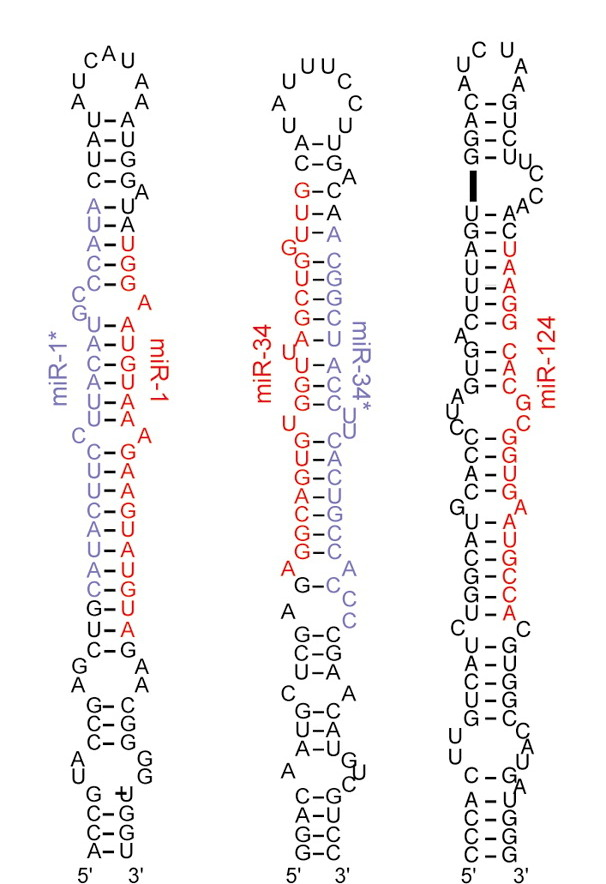
\includegraphics[width=0.4\linewidth]{figures/premiRNA_structure.png}
  \caption{Hairpin structure for three pre-miRNAs from \emph{C. elegans}.
  Red and gray colors indicate mature miRNAs.
  Reprinted with permission from \citep{Bartel2004}.}
  \label{fig:premirna-structure}
\end{figure}


In the cytoplasm, the ribonuclease Dicer cleaves out the loop of the hairpin
to form a 22-nt-long double-stranded miRNA:miRNA* duplex corresponding to
the stem of the hairpin \citep{Bernstein2001}.
Dicer associates with a cofactor, in humans TRBP (Tar RNA-binding protein),
which is not required for effective dicing of the pre-miRNA,
but acts to physically bridge the Dicer to an Argonaute protein
% for further miRNA processing
\citep{Chendrimada2005}.

The duplex is then bound by the Argonaute protein, in mammals one of Ago1
through Ago4, forming what is called the RNA-induced silencing complex (RISC).
The RISC is a protein complex containing Dicer, TRBP and Ago \citep{Gregory2005}.
Ago, aided by Dicer and TRBP, unwinds the strands of the duplex and retains one of
them. The retained strand is known as the guide strand (or miRNA). The other
strand, called the passenger (or miRNA*), is released and typically degraded \citep{Du2005}.
In some instances, either one of the strands can become the guide
or both can be used \citep{Czech2009}.
%Notably, the Dicer cleaving, duplex unwinding and eventual
%mRNA regulation activity are, in fact, all coupled and performed by RISC
%\citep{Gregory2005}.

Not all miRNAs are generated through this canonical pathway of microRNA
biogenesis. Some miRNAs are not dependent on Drosha, such as mirtrons, which
are cut into pre-miRNA by the spliceosome, a molecular complex responsible for
removing introns (and sometimes exons) from precursor mRNA \citep{Ruby2007}. The
biogenesis of miR-451 is independent of Dicer; miR-451, which
has an important role in erythropoiesis, is cleaved by Ago2 \citep{Cheloufi2010}.

\begin{figure}[htb]
  \centering
  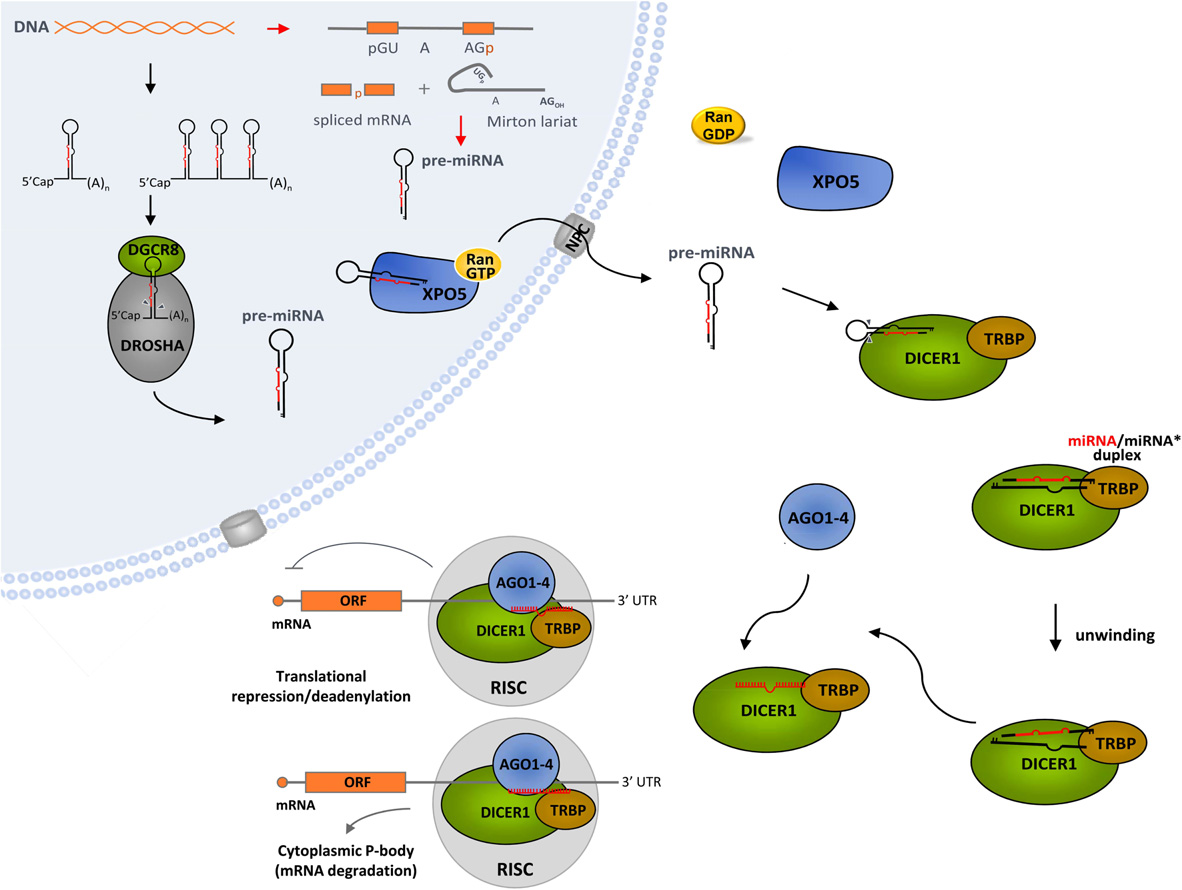
\includegraphics[width=1\linewidth]{figures/miRNA_biogenesis.png}
  \caption{Depiction of the canonical (and mirtron) pathway of microRNA biogenesis
  and microRNA mechanism of action. Figure reprinted from Melo and Esteller \citep{Melo2011}.}
  \label{fig:mirna-biogenesis}
\end{figure}




\subsection{MicroRNA mechanism of action}\label{microrna-mechanism}

The RISC is the effector of RNA interference. Ago functions as the catalytic
engine of the RISC and the miRNA bound to it guides the RISC to target
messenger RNAs \citep{Filipowicz2008}. Figure \ref{fig:mirna-biogenesis}
illustrates a rough outline of how miRNAs act to regulate mRNA expression.

Target recognition is based on sequence complementarity of the miRNA and mRNA.
In animal miRNAs this complementarity is almost always limited \citep{Ambros2004}.
Nucleotides at positions 2-8 of the 5' end of the microRNA have been found
crucial to target mRNA matching; these nucleotides are termed the miRNA "seed sequence".
miRNA target sequences are mostly located in the 3' UTR (untranslated region)
of the mRNA transcript, but in some instances target sites also reside in the
coding region or 5' UTR of the mRNA \citep{Bartel2009}.
\textbf{TÄÄ KAPPALE PAREMMIN, MUITA FIITSUJA MUKAAN, KOSKA NIITÄ KÄYTETÄÄN PREDICTIOSSA, KTS GRIMSON.)}

The action of microRNAs is \textbf{related} through inhibition of mRNA
translation or destabilization and subsequent degradation of mRNA. The exact
mechanisms by which the miRNA and Ago induce translational repression or
destabilization of mRNA are unclear \citep{Filipowicz2008}. Translational
inhibition was earlier believed to be the major form of miRNA action in animals,
but recent evidence suggests that mRNA destabilization dominates \citep{Guo2010}.
In some cases the mRNA is directly cleaved by Ago. Ago2 is the only mammalian
Argonaute capable of cleavage, and this is assumed to require
extensive base-pair matching between the miRNA and mRNA \citep{Du2005}.
However, mRNA cleavage appears to be rare in animals (while much more common
in plants).

mRNAs bound to RISC accumulate in so called processing bodies (P-bodies),
which are known sites of mRNA catabolism and translational repression in the
cytoplasm. The localization in P-bodies, however, appears to be a consequence
of RNA silencing, not the cause, and is reversible  \citep{Eulalio2007}.

Interestingly, several alternative mechanisms of action for microRNA have been
reported. For example, some miRNAs can increase the translation of target mRNA instead of
repressing it \citep{Vasudevan2007}, miR-373
was found to target DNA promoter areas and act to induce gene transcription
\citep{Place2008}, and miR-328 targets a protein to prevent inhibition of mRNA
translation \citep{Eiring2010}. This illustrates the complexity and diversity of
microRNA biology and gene regulation in general.




\subsection{MicroRNA function}\label{microrna-function}

SIIRRÄ TÄMÄ AIEMMAKSI?

MicroRNAs have been found to participate in regulation of almost all studied
cellular processes, including embryo development, cell proliferation,
apoptosis and metabolism, by regulating protein expression \cite{}.

miRNAs assert extensive control over the transcriptome. More than 60\% of
human mRNA transcripts are predicted to be regulated by miRNAs and a single
transcript has target sites for several different miRNA families
\citep{Friedman2009}. Furthermore, a single microRNA can have as many as hundreds or
thousands of target mRNAs. The effect of a
single miRNA on its target tends to be subtle, usually causing less than a
2-fold change in protein expression \citep{Baek2008}. However, a single
miRNA can have multiple binding sites in one mRNA and multiple miRNAs
acting on the same target have additive, and in some cases even synergistic
effects \citep{Bartel2009}.

% , and depending also on 
% of multiple miRNAs acting in tandem can, however, be much more pronounced and
% even multiplicative, achieving changes in excess of 10-fold \citep{}.

% A recent review concluded that mRNA degradation is the
% predominant form of miRNA action in mammals \citep{Guo2010}.

It should be noted, however, that the functional role and importance of many
miRNA-mRNA interactions are unknown, even for validated interaction pairs.
Uncovering these roles is challenging because of the subtle regulatory effects
that miRNAs often have and, additionally, because of the complexity and
robustness of most cellular regulatory networks \citep{Bartel2009}.
Furthermore, experimentally validated target mRNAs exist only for a subset of
all known microRNAs. Nonetheless, discovering miRNA targets is a critical
step in understanding their function.

The dysregulation of microRNAs is associated with many human diseases
\citep{Jiang2009,VAIHDATÄMÄREFE}. The first example of such an association was, in
fact, found in cancer, when miR-15 and miR-16 were found to be suppressed in
chronic lymphocytic leukemia \citep{Musilova2015}. A disease-promoting role
for miRNAs has since been implicated in many different cancers, including
breast cancer \citep{Melo2011}.




\subsection{Measuring MicroRNA expression}

The same methods that have been employed for measuring mRNA (i.e. gene)
expression are generally applicable for measuring microRNA expression as well,
ranging from northern blotting to microarrays and more recent studies using next
generation sequencing (NGS) \citep{Huang2011}. However, as Hunt and colleagues
in a recent and thorough review point out, there are several challenges in
detecting miRNAs in particular \citep{Hunt2015}.

MicroRNAs are very short and only comprise approximately 0.01\% of RNA
typically extracted from a sample \citep{Dong2013}. This implies that miRNA
detection must be highly sensitive. MicroRNAs from the same family can differ
by only one base, which in turn requires high specificity to be able to
distinguish between family members. On the other hand, variation in miRNA
processing can result in slight sequence variations, or isoforms, of a single
miRNA, also known as isomiRs \citep{StaregaRoslan2011,Lee2010}. This means
high specificity or an incorrect reference sequence (e.g. that of a
weakly-expressed isomiR) used for detection can cause inaccurate measurements.
IsomiRs may also have different functions resulting from altered target
specificity \citep{Chugh2012}. The existence of the pri-miRNA, pre-miRNA and
mature miRNA molecules provides an additional challenge for measurement
methods.
%, although differentiation between these maturation stages is not necessarily required.

Many of the challenges mentioned are solved by NGS, which is sensitive and
reliable in quantifying known microRNAs and identifying novel ones
\citep{Huang2011}. Sequencing can detect variations of even one nucleotide and
does not necessarily depend on previously identified sequences. However, not
all identified short RNAs are functional miRNAs, and NGS conveys its own set
of problems relating to high cost, significant computational complexity and
validation efforts to distinguish relevant data from noise
\citep{Chugh2012,Hunt2015}.

\textbf{TÄHÄN VIELÄ ERI PLATFORMIEN VERTAILUA JA PREPROSESSOINNISTA?}
